\documentclass{article}

\usepackage{amsmath}
\usepackage{amsfonts}
\usepackage{amssymb}
\usepackage{amsthm}
\usepackage{amsrefs}
\usepackage[spanish, mexico]{babel}
\usepackage[margin=0.5in]{geometry}
\usepackage[utf8]{inputenc}
\usepackage{endnotes}
\usepackage{graphicx}
\graphicspath{ {images/} }

\begin{document}
	\title{Taller X}
	\author{Leidy C. Sánchez, Miguel A. Gómez}
	\maketitle
	
	\paragraph{1.} Reproduzca y explique en completo detalle todas las soluciones presentadas para el problema del juego de cartas, incluyendo el que tiene congruencias.
	
	\paragraph{Problema de un juego de naipes} Un juego especial de naipes se compone de $n$ cartas. Si se distribuye equitativamente entre 7 jugadores queda una carta. Si se distribuye entre 11 jugadores quedan 10 cartas.
	¿Cuáles son los posibles valores de $n$?. ¿Cuál es la mínima cantidad de cartas que tiene el juego de naipes? 
	
	\paragraph{Explicación en detalle de la primera solución} Como n es la incógnita, se puede construir un sistema de ecuaciones lineales. Para el primer caso, las cartas se distribuyen entre 7 jugadores y como queda una carta de más, se resta el 1:
	
	$$n-1=7t$$
	
	Lo mismo para el segundo caso, pero quedan 10 cartas:
	
	$$n-10=11s$$
	
	con $t$ y $s \in \mathbb{Z}$. Este sistema de ecuaciones lineales puede convertirse en un sistema de congruencias lineales, de tal modo que
	
	$$n\equiv 1 \pmod{7}$$
	$$n\equiv 10 \pmod{11},$$
	
	de la primera congruencia, $n=7s+1$ y se reemplaza en la segunda congruencia, así:
	
	$$7s+1\equiv 10 \mod{11}$$ 
	
	que es lo mismo que
	
	$$7s\equiv9\mod{11}.$$
	
	Nótese que al multiplicar esta congruencia por 8, se tiene que $56\equiv 1 \pmod{11}$ y como $56s\equiv11\pmod{11}$, se puede concluir por la propiedad 3\footnote{Si $a \cdot b \equiv c \pmod{n}$ y $a \equiv s \pmod{n}$, entonces $s \cdot b \equiv c \pmod{n}$ } descrita en el documento, que $s\equiv72\pmod{11}$, pero $72\equiv6\pmod{11}$, por lo tanto, $s\equiv6\pmod{11}$, entonces por definición de congruencias, se sigue que $s=6+11t$ y ya este valor se puede reemplazar en la ecuación $n=7s+1$, así
	
	$$n=43+77t$$
	
	donde el mínimo valor que puede tomar $n$ se presenta cuando $t$ equivale a cero, de manera que este valor es 43 y es la mínima cantidad de cartas que puede tener el juego. Para determinar los otros valores que puede tner $n$, basta con asignarles valores a $t, t>0$. 
	
	\paragraph{Explicación en detalle de la segunda solución}
	Del sistema de congruencias que se pleanteó en la primera solución, se sabe que $n=7s+1$ y $n=11k+10$. Se dan valores a $s$ y a $k$ para calcular cuáles son los valores que dejar residuo 1 al dividirlos en 7 y residuo 10 al dividirse en 11 respectivamente. Por ejemplo, los primeros valores de $n$ de la primera ecuación serían
	$$\text{Si } s=0, n=1,$$
	$$\text{si } s=1, n=1,5$$
	$$\text{si } s=2, n=22,$$
	$$\text{si } s=3, n=29,$$
	$$...,$$
	
	y se efectúa el mismo procedimiento para la segunda ecuación. Seguido de esto, se comparan los valores de $n$ obtenidos de la primera y segunda ecuación, buscando soluciones en común (que sean iguales), se encuentra que el primer valor igual es $n=43$, siendo este valor la mínima cantidad de cartas que tiene el juego de naipes. Para encontrar otros valores de $n$, se busca otro valor que sea igual para ambos casos, por ejemplo se encuentra el 197, el 274 y así sucesivamente.
	
	\paragraph{Explicación en detalle de la tercera solución}
	Como $n=7s+1$ y $n=11k+10$ (resultados explicados en la primera solución), al igualar $n$ se obtiene 
	
	$$7s+1=11k+10$$
	
	donde la idea es encontrar valores de $s$ y $k$ tal que satisfagan la igualdad. Se comienzan a dar valores de manera ordenada $(1, 2, 3, ..., r)$ a $s$ y a $k$ y se comparan los resultados. Por ejemplo cuando $s=17$ y $k=10$, $n=120$ en ambos casos, pero cuando se comparan todos los valores, el mínimo valor que puede obtener $n$ es 43 cuando $s=6$ y $k=3$, siendo 43 la respuesta a la segunda pregunta del problema. Cuando se siguen comparando los valores cumpliéndose la igualdad, se tiene que $n$ puede ser 120, 197, etc. Recuerde que $n$ debe ser un entero positivo. 
	
	\paragraph{Explicación en detalle de la cuarta solución} Al igualar $n$, tal como se hizo en la tercera solución, se tiene que $7s+1=11k+10$, $7s=11k+9$ y $s=\frac{11k+9}{7}$. Esta es una ecuación lineal en la que la variable $s$ depende de los valores que toma $k$. Como se trata de una recta, se pueden asignar dos valores a $k$, por ejemplo 0 y -1 para encontrar su par ordenado y se traza la recta; al graficarse, se obtiene una recta como la siguiente:
	
	\begin{center}
		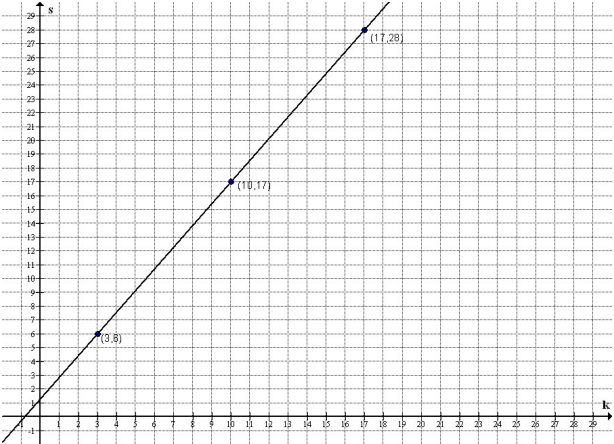
\includegraphics[scale=0.8]{Graf.PNG}
	\end{center}
	
	Como $n$ es un número entero positivo, se tienen en cuenta sólo los pares ordenados $(k,s)$ que dan un valor entero positivo en $n$, como lo son (3,8), (10, 17), (17,28), etc., arrojando valores de 43, 197, 274, etc., respectivamente.
	
	\paragraph{2.} Reproduzca y explique en completo detalle las soluciones presentadas para el problema de los soldadps de Han Xing.
	
	\paragraph{Problema de los soldados de Han Xing}¿Cuántos soldados puede tener el ejército de Han Xing si al formarlos en tres columnas quedan dos soldados, si se ordenan en 5 columnas quedan tres soldados, y al ordenarlos en 7 columnas, quedan dos soldados? 
	
	\paragraph{Explicación en detalle de la primera solución} Sea $x$ la cantidad de soldados, el problema se puede plantear como un sistema de ecuaciones lineales, nótese que para el primer caso, tendría que encontrarse la cantidad $x$ de soldados que al quitarle 2, da 3, para que se puedan formar en tres columnas; en este orden de ideas, la ecuación estaría dada por
	
	$$x-2=3r.$$
	
	Para los otros casos, se sigue la misma lógica de la formulación de la ecuación anterior y con ello se consigue el siguiente sistema de ecuaciones:
	
	$$x-2=3r$$
	$$x-3=5s$$
	$$x-2=7t.$$
	
	Donde $r$, $s$ y $t \in \mathbb{Z}$. Este sistema de ecuaciones puede ser representado como un sistema de congruencias lineales, pues siguiendo la definición de congruencias se tiene que
	
	$$x\equiv2\pmod{3}$$
	$$x\equiv3\pmod{5}$$
	$$x\equiv2\pmod{7}$$
	
	De la primera congruencia, por definición se tiene que $x=2+3r$ y al reemplazarla en la segunda congruencia se obtiene
	$$2+3r\equiv3\pmod{5}$$
	$$3r\equiv1\pmod{5}.$$
	
	\paragraph{} Y si se multiplica esta congruencia por 2, por propiedades de congruencias se sigue que $6r\equiv2\pmod{5}.$ Por la propiedad número 3 de congruencias (descrita en el documento) y teniendo en cuenta la congruencia $6 \equiv 1 \pmod{5}$, entonces $r\equiv 1\pmod{5}$, que por definición, se puede decir que $r=2+5k.$ con $k \in \mathbb{Z}$.
	
	\paragraph{}Como ya se tiene el valor de $r$, se reemplaza en la ecuación $x=2+3r$, de tal manera que $x = 2 + 3(2 + 5k) $ y $x = 8 +15k$.
	
	\paragraph{}Este valor se reemplaza en la tercera y última congruencia, así:
	$8 +15k\equiv2\pmod{7}$ y $k\equiv 1\pmod{7}$. Por definción, se tiene que $k=1+7t$ y al reemplazarse en la ecuación $x = 8 +15k, x = 23+105k$.
	
	El mínimo valor se da cuando $k=0$ y de esta forma $x=23$, lo que significa que la mínima cantidad de soldados que puede tener Han Xing es 23 y este valor satisface todas las restricciones del problema.
	
	\paragraph{Explicación en detalle de la segunda solución} Se multiplican los valores de los módulos y en este caso $3\cdot 5\cdot 7= 105=M$
	
	Sea $m_r$ el valor del módulo de cada congruencia, se procede a hallar los $M_r$, donde $M_r=\frac{M}{m_r}$, se tiene que
	
	$$M_1=35, M_2=21 \text{ y } M_3=15.$$
	
	Así, con los valores de $M_r$ se forma el siguiente sistema de congruencias lineales:
	
	$$35u_1\equiv 1\pmod{3}$$
	$$21u_2\equiv 1\pmod{5}$$
	$$15u_3\equiv 1\pmod{7}$$
	
	Y al darle valores a $u$, se tiene que las soluciones al sistema son:
	
	$$u_1=2, u_2=1 \text{ y } u_3=1$$.
	
	Finalmente, por el Teorema Chino del Residuo, se sigue que la solución general del sistema de congruencias está dado por
	
	$$x\equiv a_1M_1u_1+a_2M_2u_2+a_3M_3u_3 \pmod{M},$$
	
	donde $a_r$ representa al residuo de cada congruencia. De esta manera, se reemplazan los valores ya calculados de $M_r$ y $u_r$, así:
	
	$$x\equiv 2\cdot35\cdot2+3\cdot21\cdot1+2\cdot15\cdot1=233 \pmod{105}.$$
	
	Como $x\equiv 233 \pmod{105}$, el primer y mínimo valor de $x$ que resuelve esta congruencia es 23, así que es válido decir que $233 \equiv 23 \pmod{105}$, lo que significa que la mínima cantidad de soldados que puede tener Han Xing es 23 y este valor satisface todas las restricciones del problema.
	
	
	\paragraph{3.}  Reproduzca y explique en completo detalle las soluciones presentadas para el problema de los piratas.
	
	\paragraph{Problema de los piratas} Una banda de 17 piratas se apodera de un botín compuesto por monedas de oro de igual valor. Deciden repartirse el botín en partes iguales y dar el resto al cocinero chino. Así, el cocinero recibirá tres monedas. Pero los piratas se pelean entre ellos y seis de ellos mueren en la riña. El cocinero recibiría entonces 4 monedas. Posteriormente ocurre un naufragio y solo 6 piratas, el cocinero y el tesoro se salvan. La nueva repartición dejaría 5 monedas de oro al cocinero ¿Cuál es la fortuna mínima que esperaría el cocinero si decide liquidar al resto de los piratas?
	
	\paragraph{Explicación en detalle de la solución} se construye el sistema de 3 congruencias,
	
	\begin{enumerate}
		\item $x \equiv 3 \pmod{17}$. Esta se construye en base a que originalmente el tesoro se debe repartir en partes iguales entre 17 piratas, y por lo cual quedan 3 monedas de oro para el cocinero.
		\item $x \equiv 4 \pmod{11}$. Esta congruencia se construye en base a los 6 piratas que mueren en la riña, $17-6 = 11$ piratas y que deja como botín al cocinero 4 monedas.
		\item $x \equiv 5 \pmod{6}$. La última congruencia la construímos con los últimos 6 piratas que quedan despues del naufragio y que deja como residuo 5 monedas del botín para el cocinero.
	\end{enumerate}
	
	Ahora procedemos a solucionar este sistema de congruencias. rescribimos la primera congruencia como una ecuación diofántica, así:
	
	$$x \equiv 3 \pmod{17} \implies x = 3 + 17s \text{, con } s \in \mathbb{Z}$$
	
	con sustituímos este valor para $x$ en la segunda congruencia y simplificamos:
	
	$$3 + 17s \equiv 4 \pmod{11} \implies 17s \equiv 1 \pmod{11}$$
	
	nos interesa conocer los valores que puede tener $s$, por lo que ahora buscamos un valor que sea múltiplo de 17 congruente a 1 módulo 11, nótese que:
	$$34 = 17(2) - 1 \implies 34 \equiv 1 \pmod{11}$$
	ahora multiplicamos por 2: $17(2)s \equiv 1(2) \pmod{11}$, por propiedades de las congruencias podemos afirmar que lo anterior implica que 
	
	$$s \equiv 2 \pmod{11} \implies s = 2 + 11k \text{, con k } \in \mathbb{Z}$$
	
	Realizamos la sustitución en $x = 3 + 17s$,
	
	$$x = 3 + 17(2 + 11k) = 3 + 34 + 187k = 37 + 187k$$
	
	este nuevo valor para $x$ lo sustituímos en la tercera congruencia, luego
	
	$$37 + 187k \equiv 5 \pmod{6} \implies 187k \equiv -32 \pmod{6}$$
	
	nótese que 
	$$32 + 4 \equiv 0 \pmod{6} \implies 4 \equiv -32 \pmod{6}$$
	
	y por la propiedad de transitividad,
	
	$$187k \equiv 4 \pmod{6}$$
	
	nuevamente nos interesa conocer los valores que puede tener $k$, por lo que buscamos un valor múltiplo de 187 congruente a 1 módulo 6, nótese que:
	
	$$187 = 6(31) + 1 \implies 187 \equiv 1 \pmod{6}$$
	
	por propiedades de las congruencias podemos afirmar que lo anterior implica que
	
	$$k \equiv 4 \pmod{6} \implies k = 4 + 6t \text{ con } t \in \mathbb{Z}$$
	
	al reemplazar este resultado en $x = 37 + 187k$ obtenemos
	
	\begin{align*}
	x &= 37 + 187(4 + 6t)\\
	&= 37 + 748 + 1122t\\
	&= 785 + 1122t
	\end{align*}
	
	por lo que como mínimo el cocinero obtendrá 785 monedas de oro si decide liquidar al resto de la tripulación.
	
	\paragraph{4.} Reproduzca y explique en completo detalle las soluciones presentadas para el problema de los huevos. Y basado en este, inventeun problema que pueda ser resuelto con una congruencia.
	
	\paragraph{Problema de los huevos} Una mujer fue al mercado y un caballo quebró los huevos que tenía en su canasto. El dueño del caballo ofreció pagarle por el daño causado. Le preguntó cuantos huevos había quebrado su caballo. La mujer dijo que no sabía, pero recordó que cuando los ordenó de dos en dos, quedaba uno. Igual cosa sucedió cuando los ordenó en grupos de 3, de 4, de 5, y de 6. Pero cuando los ordenó en grupos de 7, no quedó ninguno ¿Cuál es la mínima cantidad cantidad de huevos que había en el canasto?
	
	\paragraph{Explicación en detalle de la solución} El sistema de congruencias se compone de los  casos en los que sobraba un huevo al realizar el conteo:
	$$x \equiv 1 \pmod{2}$$
	$$x \equiv 1 \pmod{3}$$
	$$x \equiv 1 \pmod{4}$$
	$$x \equiv 1 \pmod{5}$$
	$$x \equiv 1 \pmod{6}$$
	
	Y el caso en el que no sobraban huevos al realizar el conteo:
	
	$$x \equiv 0 \pmod{7}$$
	
	podríamos realizar sustituciones sucesivas, sin embargo en este caso por propiedades de las congruencias\footnote{Si $a \equiv b \pmod{n}$ y $n = (m_1)(m_2)$, entonces $a \equiv b \pmod{m_1}$ y $a \equiv b \pmod{m_2}$.} construimos una congruencia que sea equivalente, nótese que podemos realizar esta construcción debido a que hay numeros que tienen el módulo compuesto, hay varias maneras de realizar esta construcción sin embargo el objetivo es obtener la solución que indica el autor, por lo que la construímos con las congruencias módulo $3,4$ y $5$, y obtenemos:
	
	$$x \equiv 1 \pmod{60}  \implies x = 1 + 60t \text{ con } t \in \mathbb{Z}$$
	
	sustituímos en la última congruencia
	
	$$ 1 + 60t \equiv 0 \pmod{7} \implies 60t \equiv -1 \pmod{7} \implies 60t \equiv 6 \pmod{7} \implies 10t \equiv 1 \pmod{7}$$
	
	nótese que requerimos despejar t, por lo que construímos la congruencia
	
	$$50 = 7(7) + 1 \implies 10(5) \equiv 1 \pmod{7}$$
	
	por ende, debemos multiplicar por 5 la congruencia que contiene a $t$ luego
	
	$$50t \equiv 5 \pmod{7}$$
	
	y por las propiedades de las congruencias
	
	$$t \equiv 5 \pmod{7} \implies t = 5 + 7p \text{ con } p \in \mathbb{Z}$$
	
	sustituímos en $x = 1 + 60t$ y obtenemos
	
	$$x = 1 + 60(5 + 7p) = 1 + 300 + 420p = 301 + 420p$$
	
	que implica $x \equiv 301 \pmod{420}$.
	
	\paragraph{Ejercicio} La misma mujer recibió el pago del hombre del caballo a una moneda por cada huevo, al llegar a su casa, notó que le quedaban muchas menos monedas, cierta vez un médico le dijo a la mujer que tenía deficiencia en ácidos grasos omega 3 y por eso habían momentos en los que se le olvidaban las cosas, sin embargo al repasar los eventos del día recordó que compró un nuevo canasto por 14 monedas y al contar su dinero de a 7 no le sobraba. Para mejorar su memoria decidió también comprar un poco de maní y nueces por 6 monedas, al contar su dinero de a 5 no le sobraba, tambien recordó que se le había acabado la leche de almendras y las arepas para el desayuno, luego de comprar la leche y las arepas por 4 monedas al contar de a 2 no le sobraba, también recordó que se le iban acabando los minutos y iba a llamar mas tarde a su hijo, por lo que recargó su linea prepago con 13 monedas lo cuál le pareció un abuso... al contar de a 17 le quedó sobrando una moneda. Si alcanzó a pagar todo lo anterior ¿Cuánto dinero tenía la mujer como mínimo, antes de recibir el mínimo pago de parte del hombre del caballo?
	
	\paragraph{Solución} primero debemos construir el sistema de congruencias. con la cantidad inicial de dinero y el pago de la canasta construímos:
	
	$$x - 14 \equiv 0 \pmod{7} \implies x \equiv 14 \pmod{7} \implies x \equiv 0 \pmod{7}$$
	
	Luego compró las semillas por 6 monedas:
	
	$$x - 14 - 6 \equiv 0 \pmod{5} \implies x \equiv 20 \pmod{5} \implies x \equiv 0 \pmod{5}$$
	
	Luego compró la leche y las arepas por 4 y 9 monedas respectivamente,
	
	$$x - 14 - 6 - 2 \equiv 0 \pmod{2} \implies x \equiv 22 \pmod{2} \implies x \equiv 0 \pmod{2}$$
	
	$$x - 14 - 6 - 2 - 11 \equiv 0 \pmod{17} \implies x \equiv 35 \pmod{17} \implies x \equiv 1 \pmod{17}$$
	
	resumiendo así, tenemos las congruencias:
	
	$$x \equiv 0 \pmod{7}$$
	$$x \equiv 0 \pmod{5}$$
	$$x \equiv 0 \pmod{2}$$
	$$x \equiv 1 \pmod{17}$$
	
	Por las propiedades de las congruencias, podemos construir reducirlas primeras tres congruencias del sistema a $x \equiv 0 \pmod{70} \implies x = 70a$ con $a \in \mathbb{Z}$, al reemplazar en la segunda congruencia tenemos que
	
	$$70a \equiv 1 \pmod{17}$$
	
	Queremos buscar el valor paramétrico de $a$, como el mcd$(70, 17) = 1$ utilizaremos el lema de Bezout para encontrar una congruencia que nos permita construir la congruencia $a \equiv b \pmod{17}$.
	
	$$1 = 70x + 17y$$
	
	Siguiendo el algoritmo de Euclides obtenemos
	
	$$70 = 17(4) + 2 \implies 2 = 70 - 17(4)$$
	$$17 = 2(8) + 1 \implies 1 = 17 - 2(8)$$
	
	Realizando sustituciones sucesivas y organizando
	
	\begin{align*}
	1 &= 17 - 2(8)\\
	&= 17 - (70 - 17(4))(8)\\
	&= 17 - 70(8) + 17(32)\\
	&= 17(33) + 70(-8) \implies 70(-8) \equiv 1 \pmod{17}
	\end{align*}
	
	Por lo anterior debemos multiplicar la congruencia por $-8$, luego
	
	$$70(-8)a \equiv -8 \pmod{17}$$
	
	y por transitividad
	
	$$a \equiv -8 \pmod{17} \implies a \equiv 9 \pmod{17}$$
	
	y por ende $a = 9 + 17g$ con $g \in \mathbb{Z}$. Reemplazamos en $x = 70a$
	
	$$x = 70(9 + 17g) = 630 + 1190g$$
	
	cómo la cantidad mínima que recibió  fue de 301 monedas y la cantidad mínima según lo anterior es de 630, la cantidad mínima de dinero que debe tener la mujer se obtiene de $630 - 301 = 329$, por lo que la mujer debió tener como mínimo 329 monedas.
	
	\paragraph{5.} Un entero compuesto $n$ se llama pseudoprimo siempre y cuando $n|2^n - 2$. Se puede observar existen infinitos pseudoprimos, los primeros cuatro 341, 561, 645 y 1105. Demuestre que, si $n$ es un pseudoprimo impar, entonces $M_n = 2^n - 1$ es uno aún mayor.
	
	\begin{proof}
		Si $n$ es compuesto, por definición de número compuesto, significa que es múltiplo de algun número primo $p$, es decir, es de la forma $n = dp$ con $d$ y $p \in \mathbb{Z}$.
		
		\paragraph{} Ahora es necesario realizar la demostración del siguiente teorema\footnote{Punto 7, assignment III}.
		
		\paragraph{Teorema} Si $n$ y $d$ son enteros tal que $n|d$, entonces $2^d - 1 | 2^n - 1$.
		
		\begin{proof}
			Por definición de divisibilidad, $n = md$, con $m \in \mathbb{Z}$, al reemplazaren la expresión $2^{d} + 1$, tenemos:
			
			$$2^n -1 = 2^{md} - 1$$
			
			al aplicar la identidad $x^k - 1 = (x-1)(x^{k-1} + x^{k-2} + \dots + x + 1)$ en la expresión anterior tenemos que
			
			\begin{align*}
			2^{md} - 1 &= (2^d - 1) ((2^{d})^{m - 1} + (2^{d})^{m - 2} + \dots + 2^d + 1)\\
			&= (2^d - 1) k \text{, con } k = (2^d)^{m-1} + (2^d)^{m-2} + \dots + 2^d + 1
			\end{align*}
			
			Y por lo tanto 
			
			$$2^n - 1 = (2^d - 1) - k$$
			
			y  por divisibilidad, esto es equivalente a que $2^d - 1 | 2^n - 1$
		\end{proof}
		
		Continuando con la demostración inicial, como $M_n = 2^n -1$, entonces por el teorema demostrado anteriormente, $2^d - 1 | M_n$, como $M_n$ es compuesto si $n$ es compuesto.
		
		\paragraph{} $n|2^n - 2$ se puede rescribir como $2^n \equiv 2 \pmod{n}$ y $2^n - 2 = qn$, con $q \in \mathbb{Z}$. Sin embargo nótese tambien que $2^n - 2 = 2^n - 1 - 1$, que es la forma original de un número de Merssene, y por ende $(2^n - 1) - 1 = M_n - 1 = qn$.
		
		\paragraph{} Por propiedades de los exponentes $2^{M_n - 1} = 2^{qn}$ y $2^{M_n - 1} - 1 = 2^{qn} - 1$. Utilizando la identidad derivadadel teorema binomial\footnote{$x^k - 1 = (x-1)(x^{k-1} + x^{k-2} + \dots + x + 1)$} en $2^{qn} - 1$:
		
		\begin{align*}
		2^{qn} - 1 &= (2^n - 1)((2^n)^{q-1} + (2^n)^{q-2} + \dots + 2^n + 1)\\
		&= M_n((2^n)^{q-1} + (2^n)^{q-2} + \dots + 2^n + 1)
		\end{align*}
		
		y como $2^{mn -1} - 1 = 2^{qn} - 1$, podemos divir la parte derecha de la igualdad entre $M_n$ y por ende $2^{M_n - 1} - 1 \equiv 0 \pmod{M_n} \implies 2^{M_n - 1} \equiv 1 \pmod{M_n}$ y por propiedades de las congruencias $2(2^{M_n -1}) \equiv 2(1) \pmod{M_n} \implies 2^{M_n} \equiv 2 \pmod{M_n}$ y que podemos rescribir como
		
		$$2^{M_n} - 2 \equiv 0 \pmod{M_n} \implies M_n | 2^{M_n} - 2$$
		
		por lo que $M_n$ es pseudoprimo $M_n = 2^n - 1$, $M_n$ es mayor que $n$.
	\end{proof}
	
	\paragraph{6.} Las tres apareiciones mas recientes del cometa Halley fueron en los años 1985, 1910 y 1986; la próxima será en 2061. demuestre que
	
	$$1835^{1910} + 1986^{2061} \equiv 0 \pmod{7}$$
	
	\begin{proof}
		$1835 = (7)(262) + 1$, por lo tanto $1835 \equiv 1 \pmod{7}$ y por propiedades de las congruencias $1835^{1910} \equiv 1^{1910} \pmod{7}$ es equivalente a $1835^{1910} \equiv 1 \pmod{7}$.
		
		\paragraph{} Por otra parte, el número 1986 puede escribirse como $(7)(283) + 5$, por lo tanto $1986 \equiv 5 \pmod{7}$ y por propiedades de las congruencias $1986^{2061} \equiv 5^{2061} \pmod{7}$ que es equivalente a $1986^{2061} \equiv (5^3)^{687} \pmod{7}$.
		
		\paragraph{}Nótese que $5^2 = 125 = 126 - 1$, es decir que $5^3 \equiv -1 \pmod{7}$, por propiedades de congruencias $(5^3)^{687} \equiv (-1)^{687} \pmod{7}$, que es equivalente a $(5^3)^{687} \equiv -1 \pmod{7}$ y por transitividad equivalente a que $1986^{2061} \equiv -1 \pmod{7}$. Con lo anterior por propiedades de las congruencias se sigue que
		
		\begin{align*}
		1835^{1910} + 1986^{2061} &\equiv 1 + (-1) \pmod{7}\\
		&\equiv 0 \pmod{7}
		\end{align*}
		
		y que era lo que queríamos demostrar.
		
	\end{proof}
	
	\nocite{*}
	
	\bibliography{bibliography}
	
\end{document}